% Copyright 2021 Joel Feldman, Andrew Rechnitzer and Elyse Yeager, except where noted.
% This work is licensed under a Creative Commons Attribution-NonCommercial-ShareAlike 4.0 International License.
% https://creativecommons.org/licenses/by-nc-sa/4.0/


 \begin{frame}{Table of Contents }
\mapofcontentsB{\bd}
\label{note2.4.2a}
 \end{frame}
%----------------------------------------------------------------------------------------

%----------------------------------------------------------------------------------------
\section{2.4.2 Carbon Dating}
%----------------------------------------------------------------------------------------
%----------------------------------------------------------------------------------------
%----------------------------------------------------------------------------------------

%----------------------------------------------------------------------------------------
\begin{frame}[t]
\label{note2.4.2b}
\StatusBar{1}{13}
\centering
\begin{tikzpicture}
\onslide<-2|handout:0>{\shadedraw[ ball color=C1] (0,0)arc(-90:270:5mm)node[below]{N};}\onslide<+>{}
\onslide<+>{\foreach \x in {-1,0,1}{\draw[->,W1,ultra thick] (\x,1.75)--(\x,1.25);}}
\onslide<+->{\shadedraw[ ball color=W1] (0,0)arc(-90:270:5mm)node[below]{$^{14}$C};}
\onslide<+->{\foreach \x/\y in {1/1,-1/1,-2/0,2/0}{
	\shadedraw[ ball color=gray] (\x,\y)arc(-90:270:5mm)node[below]{$^{12}$C};}}
\onslide<+-8|handout:1>{
	\index{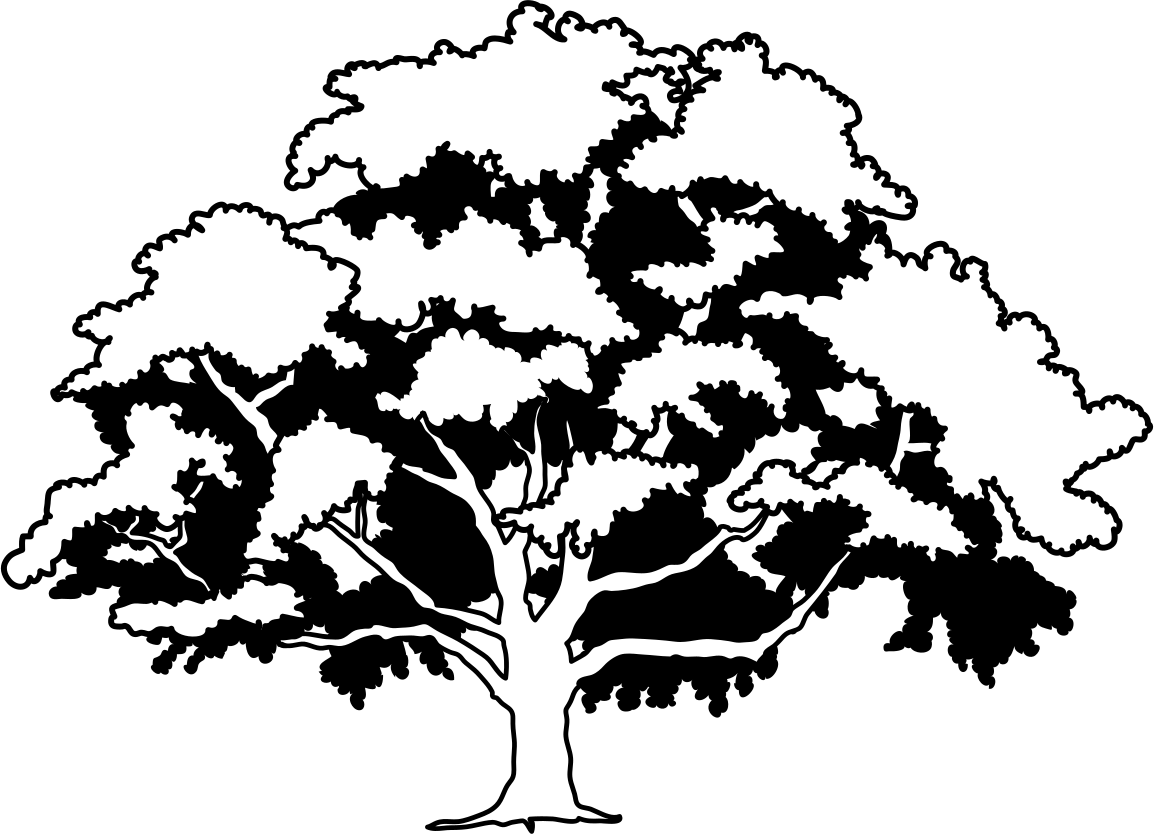
\includegraphics[height=3mm]{clipart/tree} \href{https://thenounproject.com/icon/tree-1029983/}{Tree} by \href{https://thenounproject.com/visuadio/}{Felipe Alvarado} is licensed under \CCBYthree~(accessed 10 January 2023)}
	\draw (-2,-3)node{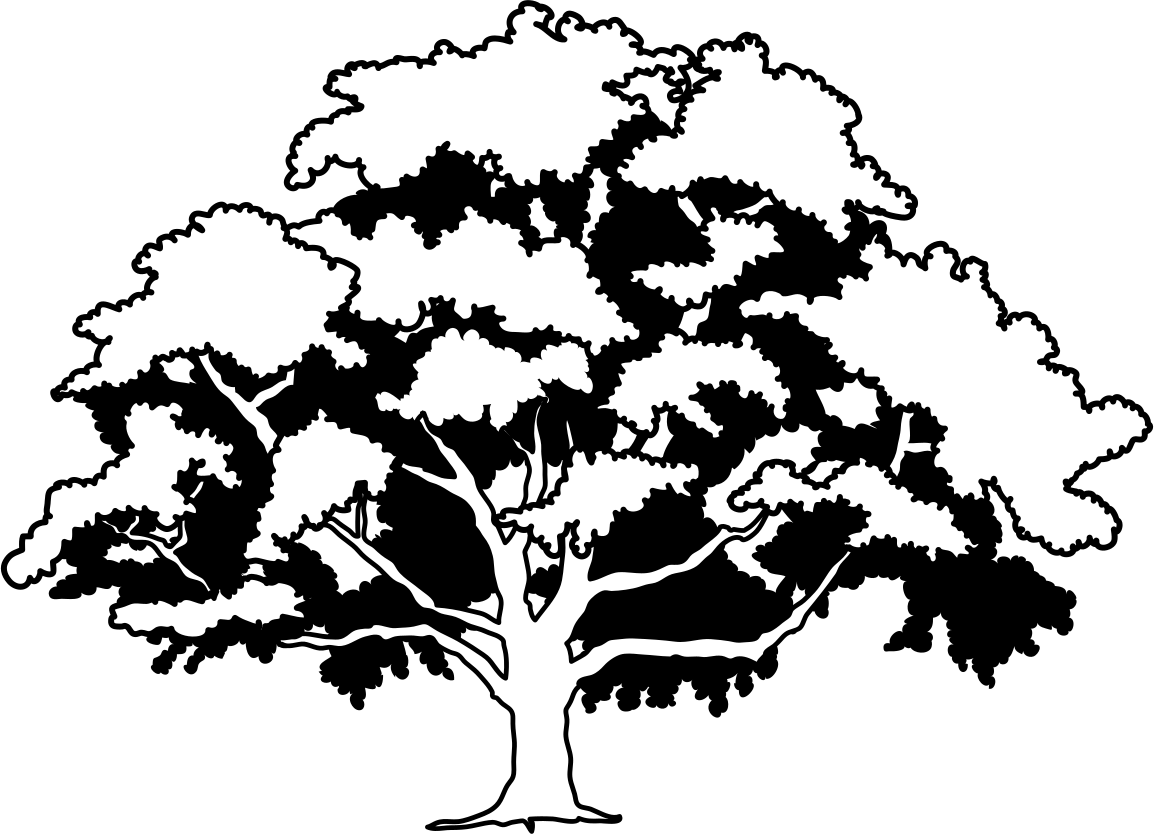
\includegraphics[height=5cm]{clipart/tree}};}
\onslide<+-8|handout:1>{
	\draw[line width=2mm,->] (-3,0)to[bend right] (-4,-1); 
	\foreach \x/\y in {-1/-1.5,-.75/-1.25,-1.5/-1.6,-.5/-1.75,-.625/-1.5,-1.2/-1.3,
		0/-2.5,-.25/-2.6,.5/-3,.25/-2.75,.74/-3.125,.6/-3.3,.6/-2.7,
		-2/-1,-2.2/-1.2,-2.5/-1,-2.75/-1.25,-3/-1.3,-3.25/-1.4
		}{
	\shadedraw[ ball color=gray,opacity=0.9] (\x,\y)arc(-90:270:1mm);}
	\foreach \x/\y in {-1/-1,0/-2.75,1/-3.25,-2.4/-1.3}{
	\shadedraw[ ball color=W1] (\x,\y)arc(-90:270:1mm);}
	}
\onslide<+-8|handout:1>{
	\index{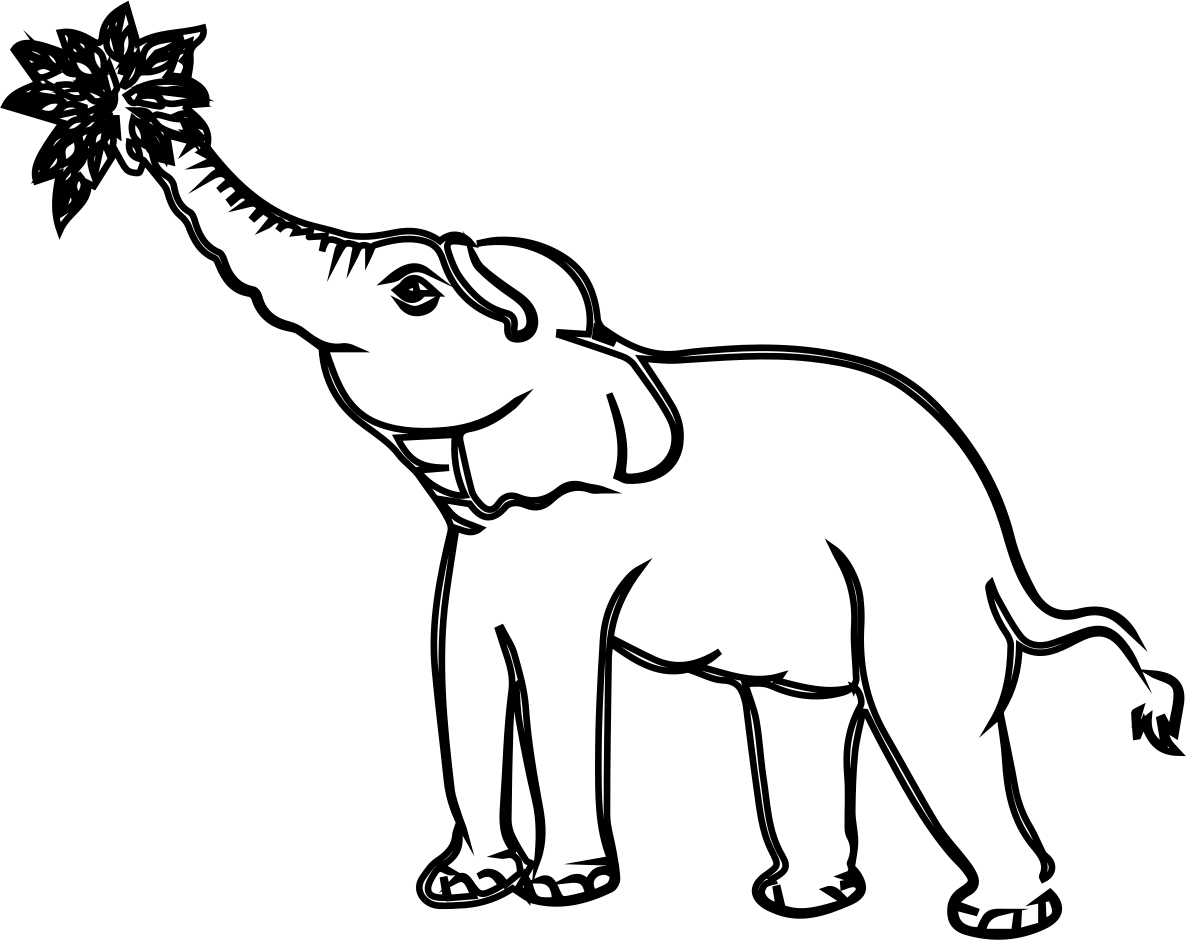
\includegraphics[height=3mm]{clipart/elephant} \href{https://thenounproject.com/icon/elephant-eating-407763/}{Elephant eating} by \href{https://thenounproject.com/paulami/}{Paulami Roychoudhury
} is licensed under \CCBYthree~(accessed 10 January 2023)}
	\draw (3,-4)node{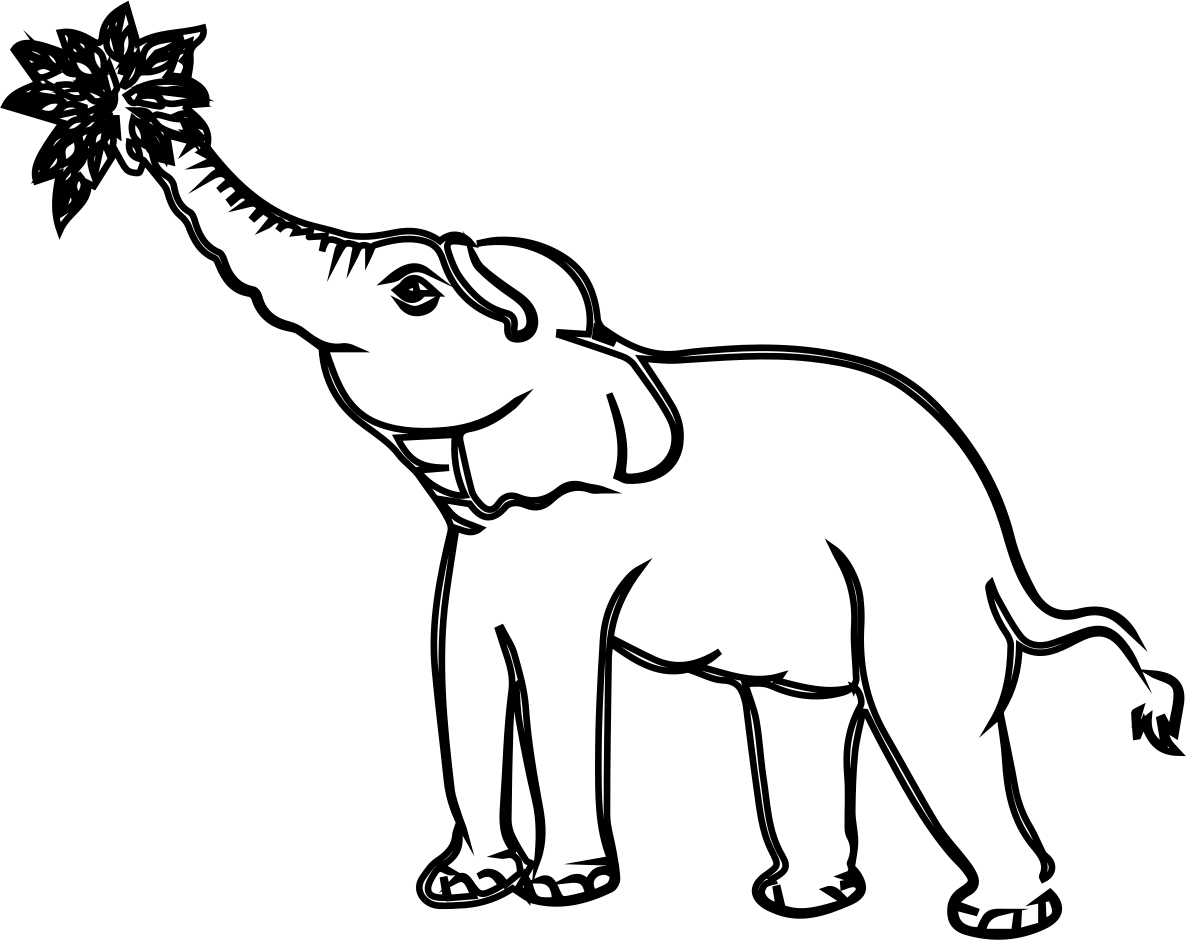
\includegraphics[width=4cm]{clipart/elephant}};}
\onslide<+-8|handout:1>{
	\foreach \x/\y in {3.25/-4.25,3.5/-4,3.6/-4.25,4.1/-4.6,4/-4.2
		}{
	\shadedraw[ ball color=gray,opacity=0.9] (\x,\y)arc(-90:270:1mm);}
	\foreach \x/\y in {3.5/-4.5}{
	\shadedraw[ ball color=W1] (\x,\y)arc(-90:270:1mm);}
	}
\begin{scope}[yshift=5mm]
\onslide<+-|handout:2>{
	\index{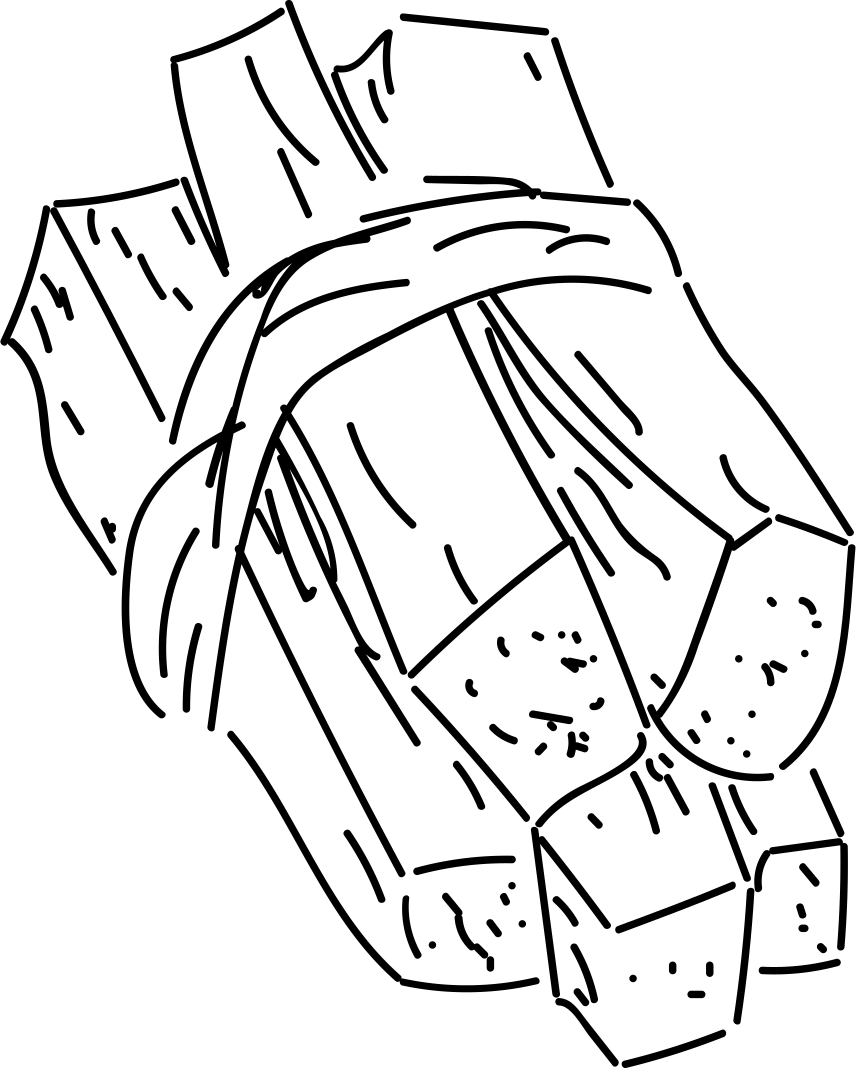
\includegraphics[height=3mm]{clipart/firewood}\href{https://thenounproject.com/icon/firewood-1301727/}{Firewood} by \href{https://thenounproject.com/alineescobar/}{Aline Escobar} is licensed under \CCBYthree~(accessed 10 January 2023)}
	\draw(0,-4)node[opacity=0.75]{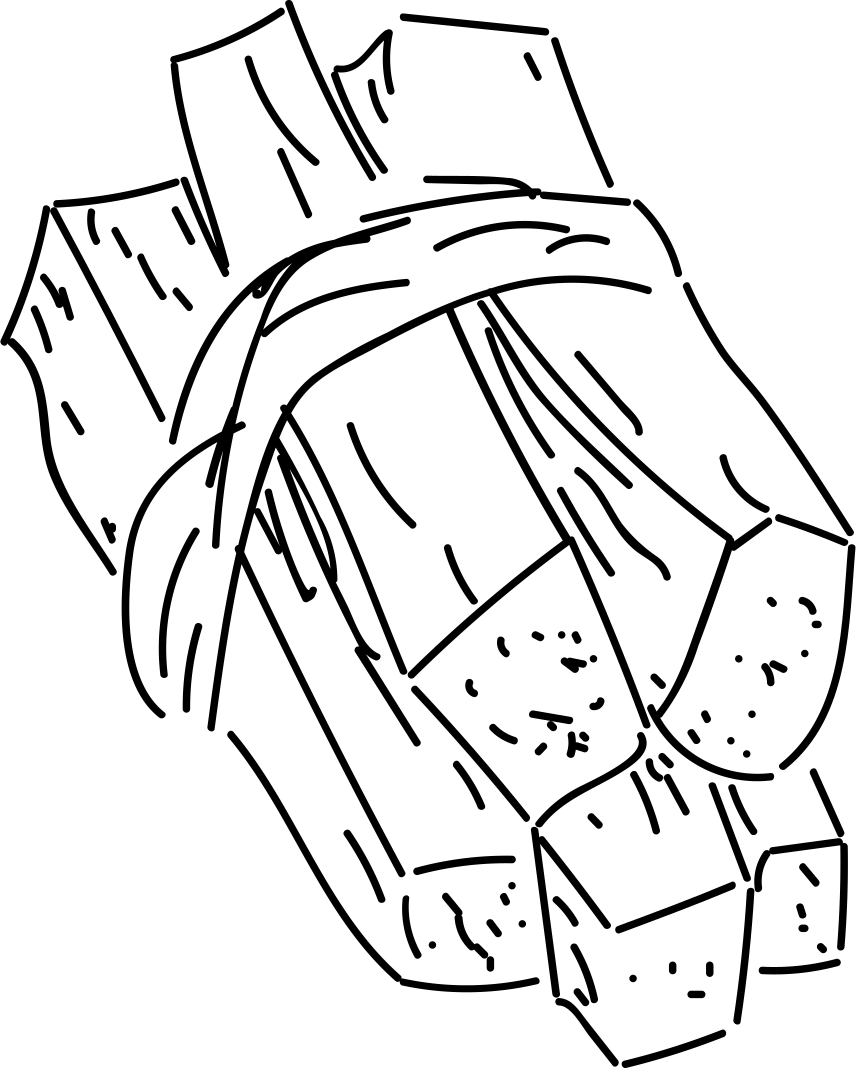
\includegraphics[width=4cm]{clipart/firewood}};}
\onslide<+-|handout:2>{
	\foreach \x/\y in {.1/-2,1/-3.1,1.2/-3.5,1.1/-4.5,
		-1/-2,-.75/-2.5,-.1/-4.5,0/-3.5,
		-1.5/-3.5
		}{
	\shadedraw[ ball color=gray,opacity=0.9] (\x,\y)arc(-90:270:1mm);}
	\foreach \x/\y in {.5/-2.25,.25/-4,-.125/-5.25,-.8/-4.8}{
	\shadedraw[ ball color=W1] (\x,\y)arc(-90:270:1mm);}
	}
\onslide<+-|handout:2>{\draw[W4](.5,-2.15)node{\huge$\times$};\draw[C2](.5,-2.15)node[rotate=45]{\huge$\times$};}
\onslide<+-|handout:0>{\draw[W4](.25,-3.9)node{\huge$\times$};\draw[C2](.25,-3.9)node[rotate=45]{\huge$\times$};}
\onslide<+-|handout:0>{\draw[W4](-.125,-5.15)node{\huge$\times$};\draw[C2](-.125,-5.15)node[rotate=45]{\huge$\times$};}
\end{scope}%firewood
\end{tikzpicture}
\end{frame}

%----------------------------------------------------------------------------------------%----------------------------------------------------------------------------------------
\begin{frame}[t]{Radioactive Decay}
One model for radioactive decay says that the rate at which an isotope decays is proportional to the amount present. So if $Q(t)$ is the amount of a radioactive substance, then
\[\diff{Q}{t}=-kQ(t)\]
for some constant\footnote{By including the negative sign, we ensure $k$ will be positive, but of course we could also write ``$\diff{Q}{t}=KQ(t)$ for some [negative] constant $K$".} $k$. 
\vfill
This is a first-order linear differential equation. Its explicit solutions have the form:
\sonslide<2->{\[ Q(t)=Ce^{-kt}\]
where $C=Q(0)$.}
\end{frame}
%----------------------------------------------------------------------------------------
\begin{frame}[t]{Half-life}
The \alert{half-life} of an isotope is the time required for half of that isotope to decay. If we know the half-life of a substance is $t_{1/2}$, and its quantity at time $t$ is given by $Q(0)e^ {-kt}$ we can find the constant $k$:

\sonslide<2->{
\begin{multicols}{2}	\begin{align*}
	\frac12 Q(0)&=Q(t_{1/2})=Q(0)e^{-kt_{1/2}}\\
	\frac12&=e^{-kt_{1/2}}\\
	2&=e^{kt_{1/2}}\\
	\log 2 & = kt_{1/2}\\
	\frac{\log 2}{t_{1/2}}&=k
	\end{align*}
	Plugging this back in gives us a more intuitive equation for the quantity of a radioactive substance over time:
	\begin{align*}
	Q(t)&=Q(0)e^{-\frac{\log 2}{t_{1/2}}t}\\
	&=Q(0)\cdot\left(\frac12\right)^{\frac{t}{t_{1/2}}}
	\end{align*}
So if $t=t_{1/2}$, the initial amount is cut in half; if $t=2t_{1/2}$, the initial amount is cut in half twice (i.e. quartered), etc.
	\end{multicols}
	}
	\vfill\color{black}
	

\end{frame}
%----------------------------------------------------------------------------------------
\begin{frame}[t]
\begin{block}{Radioactive Decay}
The function $Q(t)$ satisfies the equation
$
\diff{Q}{t} = -k Q(t)
$
if and only if
\[
Q(t) = Q(0)\, e^{-kt}
\]

The half--life is defined to be the time $t_{1/2}$ which obeys
$
Q\big(t_{1/2}\big) = \frac{1}{2}\,Q(0)
$.
The half--life is related to the constant $k$ by
$
t_{1/2} =\frac{\log 2}{k}
$. Then
\[Q(t) = Q(0)\, e^{-\frac{\log 2}{t_{1/2}}t}=Q(0)\cdot\left(\frac12\right)^{\frac{t}{t_{1/2}}}\]

\end{block}
If the half-life of $^{14}$C is $t_{1/2}=5730$ years, then the quantity of carbon-14 present in a sample after $t$ years is:
\sonslide<2->{\[Q(t)=Q(0)e^{-\frac{\log2}{5730}t}=Q(0)\left(\frac12\right)^{\frac{t}{5730}}\]}
\unote{Corollary~\eref{text}{cor:carbonDating}}
\end{frame}
%----------------------------------------------------------------------------------------
\begin{frame}[t]
\AnswerYes<1,3>
\sMoreSpace<2>
A particular piece of flax parchment contains about 64\% as
much ${}^{14}C$ as flax plants do today.
We will estimate the age of the parchment, using $5730$ years as the half-life of $^{14}$C.

\snshonly{-2}{1}{1-}{\textcolor{C3}{First, a rough estimate: is the parchment older or younger than 5730 years?}\AnswerYes}

\sonly<2>{
Younger: it has \textit{more} that half its  $^{14}$C left, so it has been decaying for \textit{less} than one half-life.
}

\sonslide<4->{
Let $Q(t)$ denote the amount of ${}^{14}C$ in the parchment
$t$ years after it was first created. 

\begin{multicols}{2}
\begin{align*}
Q(t) &= Q(0)\left(\frac12\right)^{\frac{t}{5730}}\\
0.64&=\left(\frac12\right)^{\frac{t}{5730}}\\
\log(0.64)&=\frac{t}{5730}\log \frac12=-\frac{\log 2}{5730}t\\
t&=-\frac{5730\log(0.64)}{\log 2}\approx 3689
\end{align*}
\columnbreak

\begin{align*}
Q(t) &= Q(0)e^{-\frac{\log 2}{5370}t}\\
0.64&=e^{-\frac{\log 2}{5370}t}\\
\log(0.64)&=-\frac{\log 2}{5730}t\\
t&=-\frac{5730\log(0.64)}{\log 2} \approx 3689
\end{align*}
\end{multicols}
So the parchment was made of plants that died about 3700 years ago.}
\unote{Example~\eref{text}{eg:SDEcarbonDating}}
\end{frame}
%----------------------------------------------------------------------------------------%----------------------------------------------------------------------------------------
\section{2.4.3 Newton's Law of Cooling}
%----------------------------------------------------------------------------------------
%----------------------------------------------------------------------------------------
%----------------------------------------------------------------------------------------
\begin{frame}[t]
\begin{block}{Newton's law of cooling}
The \alert<1|handout:0>{rate of change} of \alert<2|handout:0>{temperature of an object} is proportional to
the difference in temperature between the object and its \alert<3|handout:0>{surroundings}.
\end{block}
The temperature of the surroundings is sometimes called the ambient
temperature.

\begin{center}
\begin{tikzpicture}
\onslide<1>{\draw (0,0)node{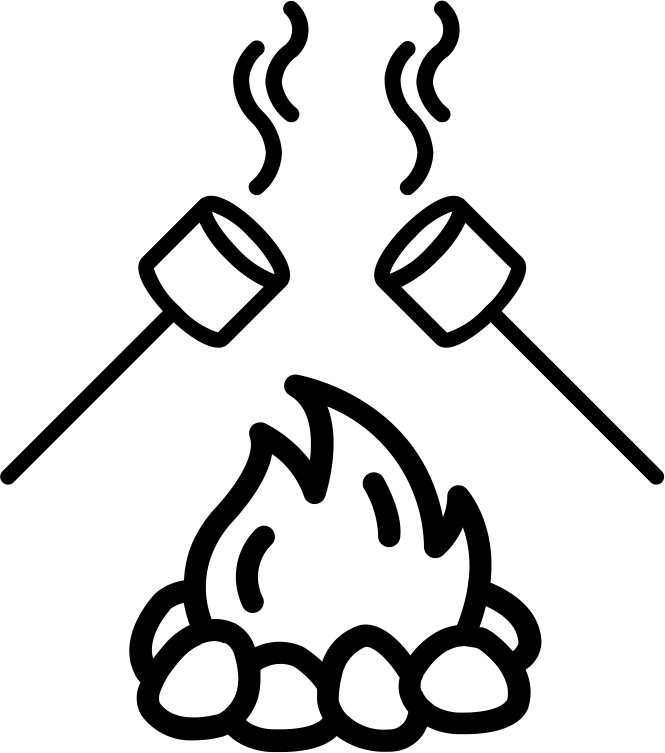
\includegraphics[width=3cm]{clipart/marshmallows}};}
\onslide<2>{\draw (0,0)node{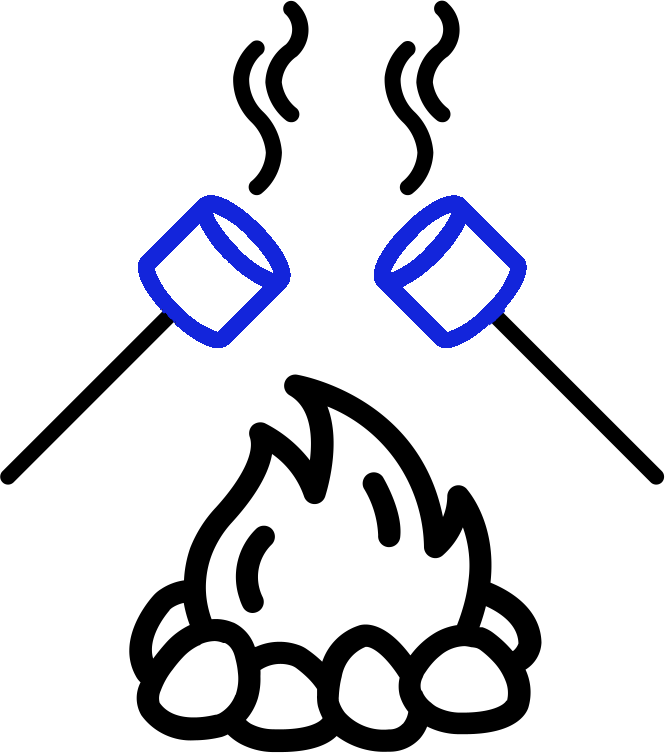
\includegraphics[width=3cm]{clipart/marshmallows1}};}
\onslide<3->{\draw (0,0)node{
\includegraphics[width=3cm]{clipart/marshmallows2}};}

\end{tikzpicture}
\end{center}
\index{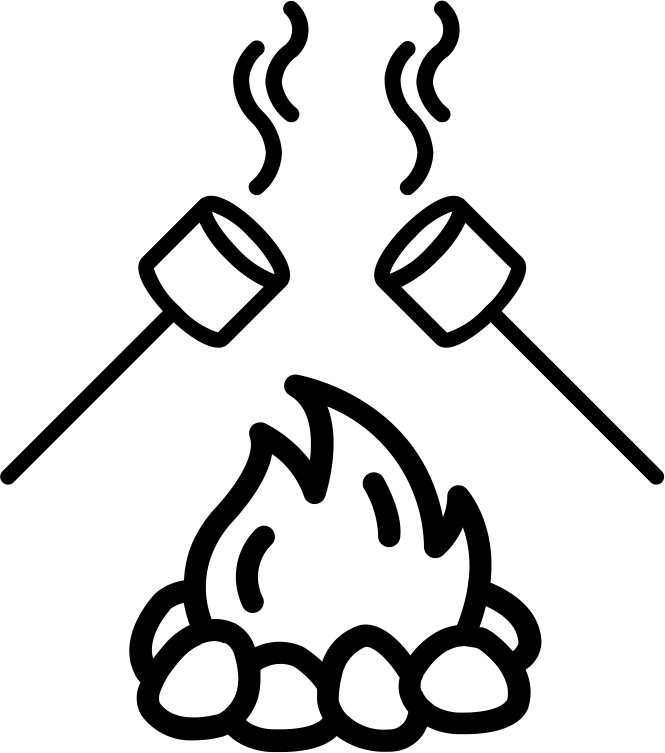
\includegraphics[height=3mm]{clipart/marshmallows} \href{https://thenounproject.com/icon/roasting-marshmallows-2602776/}{Roasting Marshmallows}  by \href{https://thenounproject.com/cgeorge1028/}{Caitlin George} is licensed under \CCBYthree~(accessed 28 August 2022; colour modified)}


\[\diff{T}{t}=\only<beamer>{K\left(\onslide<2->{\textcolor{C1}{T(t)}\onslide<3->{-\textcolor{W1}{A}}}\right)}\]
\unote{Equation~\eref{text}{eq:newtonCooling}}
\end{frame}
%----------------------------------------------------------------------------------------
\begin{frame}[t]
\NoSpace<1>\AnswerYes<1>
\begin{block}{Linear First-Order Differential Equations}
Let $a$ and $b$ be constants.
The differentiable function $y(x$) obeys the differential equation
\begin{equation*}
\diff{y}{x} =a(y-b)
\end{equation*}
if and only if
\begin{equation*}
y(x) = \{y(0)-b\}\,e^{ax} + b
\end{equation*}
\end{block}
Find an explicit formula for functions $T(t)$ solving the differential equation $\displaystyle\diff{T}{t}=K(T(t)-A)$
for some constants $K$ and $A$.

\sonslide<2->{
\[T(t)=\left(T(0)-A\right)e^{Kt}+A\]}
\end{frame}
%----------------------------------------------------------------------------------------
%----------------------------------------------------------------------------------------
\begin{frame}[t]
\label{note2.4.2c}
\NoSpace<1>\QuestionBar<1>{1}{2}\sStatusBar{1}{3}
\AnswerYes<1-2>
\AnswerBar<2->{1}{2}
\unote{Example~\eref{text}{eg:SDEcoolingA}}
%
The temperature of a glass of iced tea is initially $5^\circ$.
After 5 minutes, the tea has heated to $10^\circ$ in a room where the air
temperature is $30^\circ$.

Assume the temperature of the tea as it cools follows Newton's law of cooling,
\[T(t)=\left(T(0)-A\right)e^{Kt}+A\]
\begin{enumerate}[(a)]
\item   Determine the temperature as a function of time.
\item  When the tea will reach a temperature of $14^\circ$ ?
\end{enumerate}

\sonly<2>{
	The ambient temperature is $A=30$ and $T(0)=5$, so we only have to determine $K$. (Or, more neatly, $e^K$.)

\vspace{-7mm}
\begin{multicols}{2}
\begin{align*}
	T(t)&=\left(5-30\right)e^{Kt}+30\\&=30-25e^{Kt}\\
	10=T(5)&=30-25e^{5K}\\
	25e^{5K}&=20\end{align*}\columnbreak

	\begin{align*}
	e^{5K}&=\frac{4}{5}\\
	e^{K}&=\left(\frac{4}{5}\right)^{1/5}\\
	T(t)&=30-25\left(\frac{4}{5}\right)^{\frac{t}{5}}\\
	\end{align*}\end{multicols}
	}
\sonly<3>{
\begin{multicols}{2}
	\begin{align*}
	14=T(t)&=30-25\left(\frac{4}{5}\right)^{\frac{t}{5}}\\
	25\left(\frac{4}{5}\right)^{\frac{t}{5}}&=16\\
	\left(\frac{4}{5}\right)^{\frac{t}{5}}&=\frac{16}{25}=\left(\frac45\right)^2\end{align*}\columnbreak
	
	\begin{align*}
	\frac{t}{5}&=2\\
	t&=10
	\end{align*}
	
	After 10 minutes
	\end{multicols}
	}
\end{frame}

%----------------------------------------------------------------------------------------
%----------------------------------------------------------------------------------------
\begin{frame}[t]
\AnswerYes<1>\NoSpace<1>\QuestionBar<1>{2}{2}
\AnswerBar<2->{2}{2}
A glass of room-temperature water is carried out onto a balcony from an
apartment where the temperature is $22^\circ$C. After one minute the water has
temperature $26^\circ$C and after two minutes it has temperature $28^\circ$C.
Assuming the water warms according to Newton's law of cooling, what is the outdoor temperature?

Assume that the temperature of the water obeys Newton's law of cooling.
 
\vspace{-7mm}
\sonslide<2->{
\begin{multicols}{2}
\begin{align*}
 T(t)&=A+\big(T(0)-A\big)e^{Kt}\\
 &=A+\big(22-A\big)e^{Kt}\\
\text{Given:}\quad 26 &=A+\big(22-A\big)e^{K} \\
\implies e^K&=\frac{26-A}{22-A}\\
\text{Given:}\quad 28&=A+\big(22-A\big)e^{2K} \\
\implies e^{2K} &= \frac{28-A}{22-A}
\end{align*}\columnbreak

\begin{align*}
 \frac{28-A}{22-A}&=\left(e^K\right)^2=\left(\frac{26-A}{22-A}\right)^2\\
 (28-A)&(22-A)=(26-A)^2\\
 28\cdot22-50&A+A^2=26^2-52A+A^2\\
 2A&=26^2-28\cdot 22\\
 A&=(26)(13)-(22)(14)\\
 & =(26)(13)-(22)(13)-22\\
 &=4\cdot 13-22=30
\end{align*}
\end{multicols}
}

\unote{Example~\eref{text}{eg:SDEcoolingB}}
\end{frame}
%----------------------------------------------------------------------------------------%----------------------------------------------------------------------------------------
\section{2.4.4 Population Growth}
%----------------------------------------------------------------------------------------
%----------------------------------------------------------------------------------------

%----------------------------------------------------------------------------------------
\begin{frame}[t]
\AnswerYes<1>
Let $P$ the the size of a population, and let $K$ be the carrying capacity of its environment (i.e. the population size that can be sustainably supported).

\vfill
\begin{multicols}{2}
When $P$ is much less than $K$, our population has...
\begin{enumerate}[A.]
\item not enough resources
\item just enough resources
\item \salert<2>{extra resources}
\end{enumerate}
\columnbreak
So when the $P$ is much less than $K$, we expect the population to...
\begin{enumerate}[A.]
\item shrink
\item stay the same
\item \salert<2>{grow}
\end{enumerate}
\end{multicols}
\pause
\begin{block}{Malthusian growth}
The Malthusian growth model relates population growth to population size:
\[\diff{P}{t}=bP(t)\]
where $b$ is a constant representing net birthrate per member of the population.\end{block}
\end{frame}
%----------------------------------------------------------------------------------------%----------------------------------------------------------------------------------------
\begin{frame}[t]
\AnswerSpace
\only<1>{\AnswerYes}
Let $P$ the the size of a population, and let $K$ be the carrying capacity of its environment (i.e. the population size that can be sustainably supported).


\begin{multicols}{2}
When $P$ is \alert{greater} than $K$, our population has...
\begin{enumerate}[A.]
\item \salert<2>{not enough resources}
\item just enough resources
\item extra resources
\end{enumerate}
\columnbreak
So when the $P$ is greater than $K$, we expect the population to...
\begin{enumerate}[A.]
\item \salert<2>{shrink}
\item stay the same
\item grow
\end{enumerate}
\end{multicols}
\pause

\sonly<beamer>{\color{spoilercolor}
The Malthusian growth model 
\[\diff{P}{t}=bP(t)\]
 is \alert{not} a good model for populations with strained resources}
 \end{frame}
%----------------------------------------------------------------------------------------
%----------------------------------------------------------------------------------------
\begin{frame}
\alert{Logistic growth} models population growth as:
\[\diff{P}{t}=b_0\left(1-\frac{P(t)}{K}\right)P(t)\]
\pause

\begin{multicols}{2}
\begin{itemize}[<+->]
\item If $P<<K$, then $\diff{P}{t}\approx \onslide<+-|handout:0>{b_0P(t)}$
\item If $P\approx K$, then $\diff{P}{t}\approx \onslide<+-|handout:0>{0}$
\item If $P> K$, then $\diff{P}{t}\onslide<+-|handout:0>{< 0}$
\end{itemize}\columnbreak

\hfill\begin{tikzpicture}
\onslide<2-5>{
	\draw (7,3)node{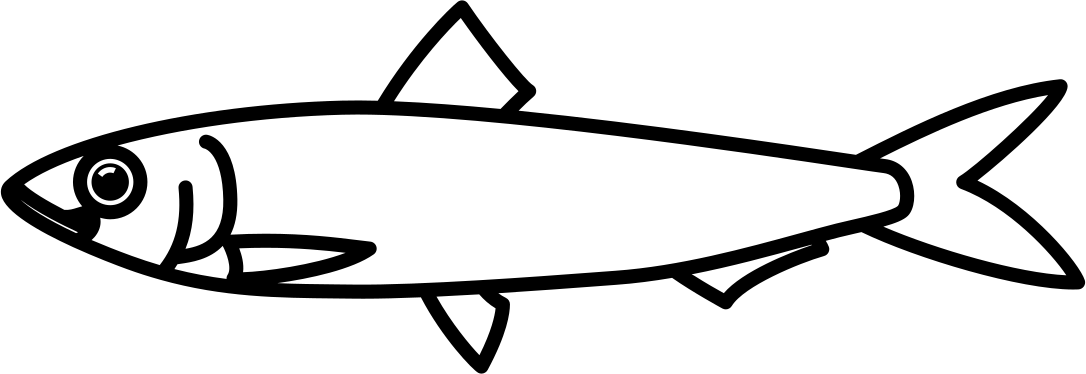
\includegraphics[width=1cm]{clipart/sardine}};
	\draw (8,2.5)node[xscale=-1]{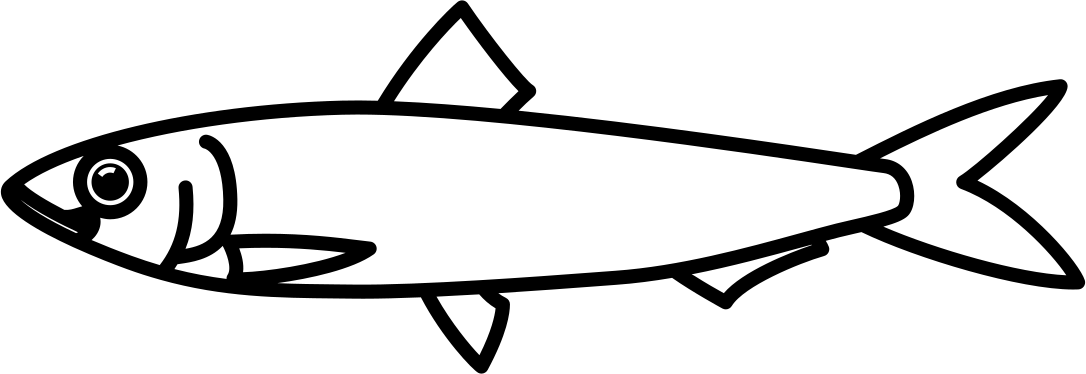
\includegraphics[width=1cm]{clipart/sardine}};}
\onslide<4-5|handout:0>{
	\draw (9,3)node{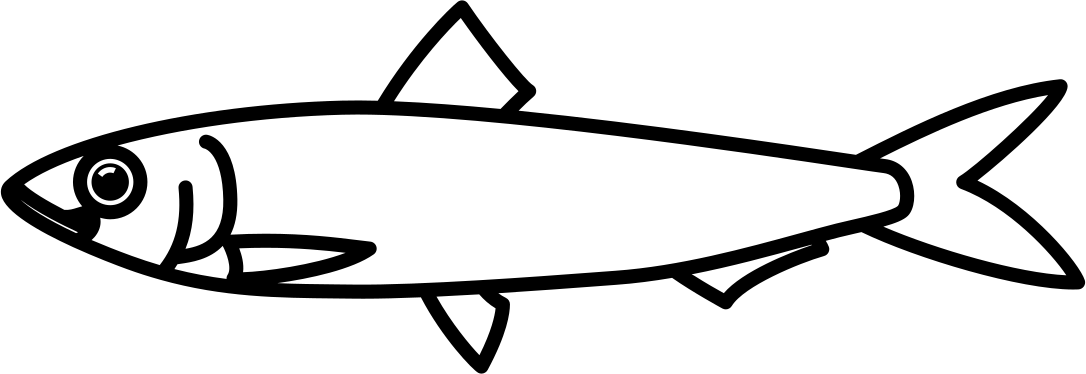
\includegraphics[width=1cm]{clipart/sardine}};
	\draw (10,2.5)node[xscale=-1]{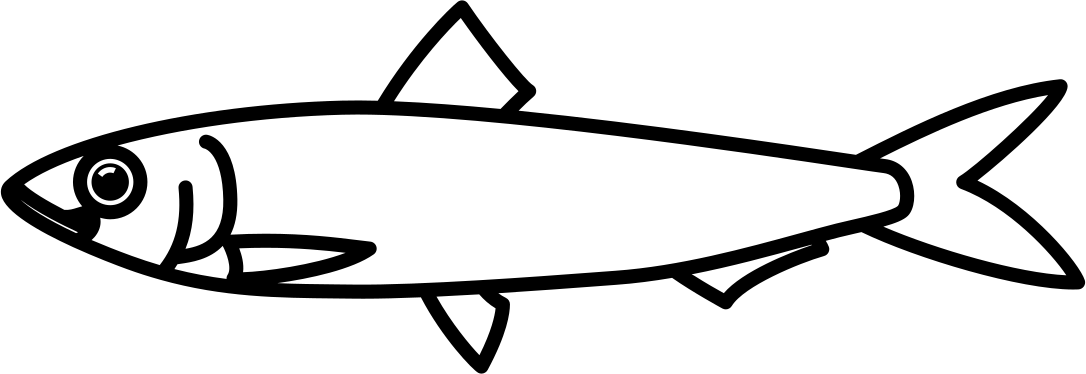
\includegraphics[width=1cm]{clipart/sardine}};
	\draw (7,2)node{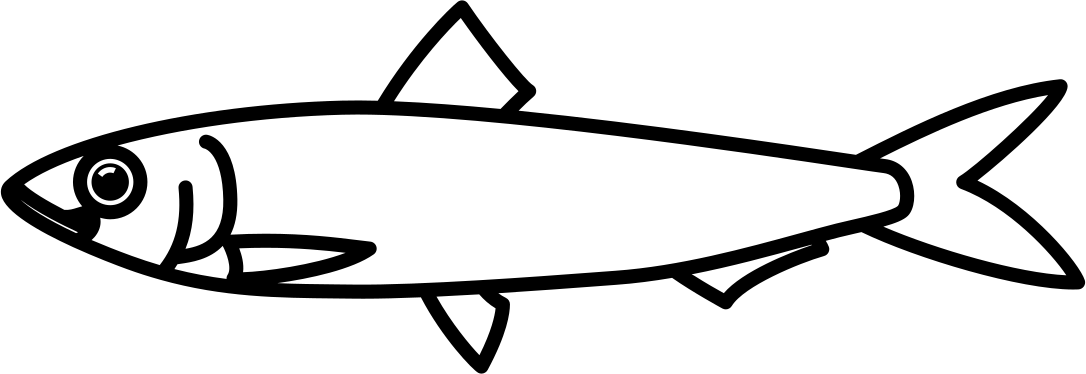
\includegraphics[width=1cm]{clipart/sardine}};
	\draw (9,2)node{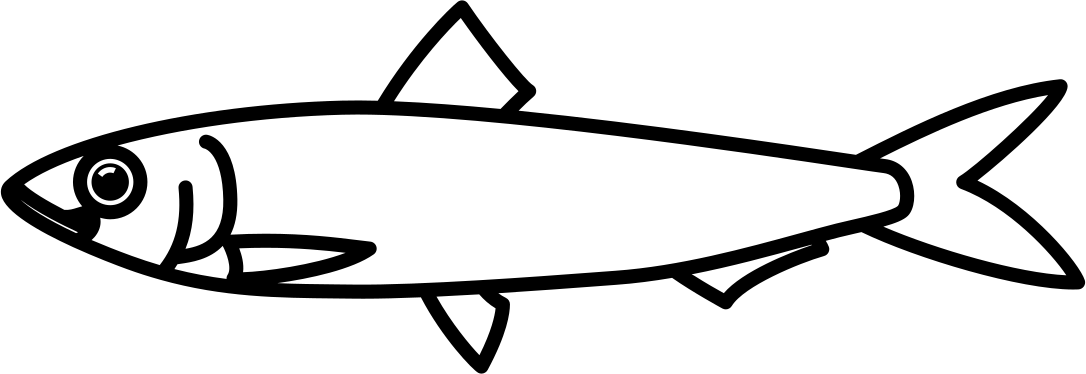
\includegraphics[width=1cm]{clipart/sardine}};
}
\onslide<6-|handout:0>{
	\foreach \x in {7,...,9}{
		\foreach \y in {0,...,5}
		{
		\DIVIDE{\y}{3}{\ya}
		\ADD{1.5}{\ya}{\yb}
		\ifodd \y \draw (\x,\yb)node[xscale=-1]{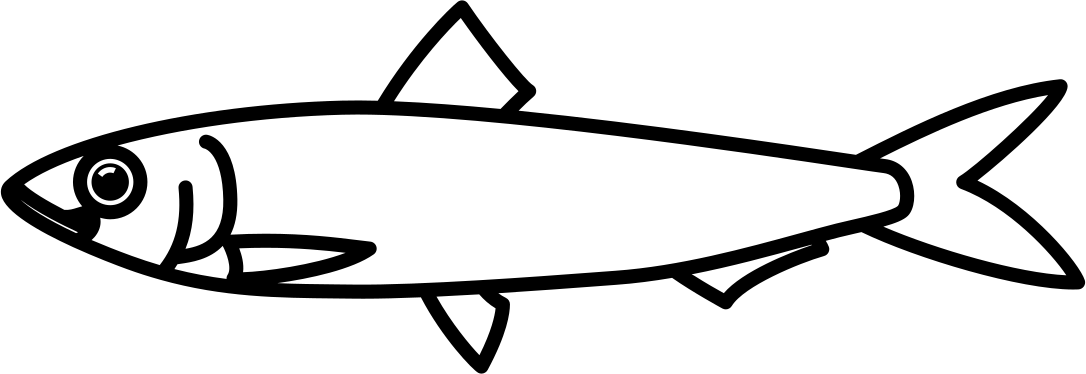
\includegraphics[width=1cm]{clipart/sardine}};
		\else \draw (\x,\yb)node{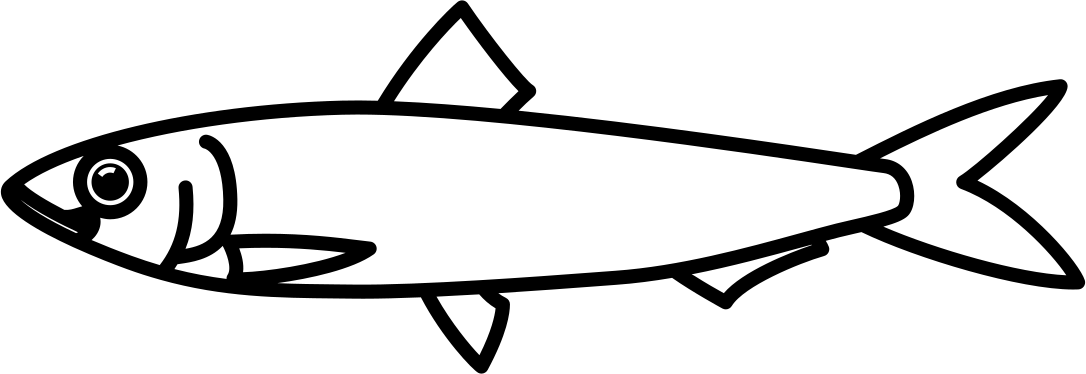
\includegraphics[width=1cm]{clipart/sardine}};
		\fi
		}}
	}
\end{tikzpicture}

\end{multicols}
\index{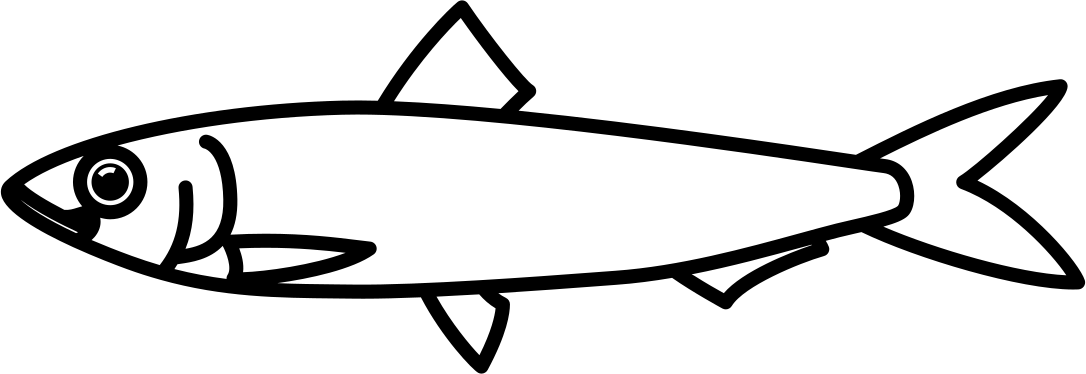
\includegraphics[height=3mm]{clipart/sardine} \href{https://thenounproject.com/icon/sardine-1630520/}{sardine} by \href{https://thenounproject.com/jbserra/}{Jaime Serra}is licensed under \CCBYthree~ (accessed 28 August 2022) }
\end{frame}

%----------------------------------------------------------------------------------------
%-------------------------------------------------------------
\begin{frame}
Before we solve explicitly, let's sketch some solutions to
\[\diff{P}{t}=b_0\left(1-\frac{P(t)}{K}\right)P(t)\]

\begin{multicols}{2}
\onslide<+->{\begin{itemize}[<+->]
\item If $P(a)=0$: \onslide<+-|handout:0>{$\diff{P}{t}=0$}
\item\color{M3} If $0<P(a)<K$: \onslide<+-|handout:0>{$\diff{P}{t}(a)>0$}
\item If $P(a)=K$: \onslide<+-|handout:0>{$\diff{P}{t}(a)=0$}
\item\color{W1} If $K<P(0)$: \onslide<+-|handout:0>{$\diff{P}{t}(a)<0$}
\end{itemize}}
\end{multicols}
\begin{center}
	\begin{tikzpicture}
	\myaxis{t}{0}{4}{P}{0}{3.2}
	\ycoord{2}{K} 
	\only<beamer>{
	\onslide<-9>{\xcoord{1}{a}}
	\onslide<2-9>{\draw (1,0)node[vertex]{};}
	\onslide<3-10>{\draw[thick] (.75,0)--(1.25,0);}
	\onslide<11->{\draw[thick] (0,0)--(4,0);}
	\color{M3}
	\onslide<4-9>{\draw (1,1)node[vertex]{};}
	\onslide<5-10|handout:0>{\draw[thick](.75,.9)--(1.25,1.1);}
	\onslide<11->{\draw[thick]plot[domain=0:4](\x,{0.75*exp(\x)/(1+.375*exp(\x))});}
	\color{black}
	\onslide<6-9>{\draw (1,2)node[vertex]{};}
	\onslide<7-10|handout:0>{\draw[thick](.75,2)--(1.25,2);}
	\onslide<11->{\draw[thick]plot[domain=0:4](\x,{20*exp(\x)/(1+10*exp(\x))});
	\draw[thick]plot[domain=0:4](\x,{-20*exp(\x)/(1-10*exp(\x))});}
	\color{W1}
	\onslide<8-9>{\draw (1,3)node[vertex]{};}
	\onslide<9-10|handout:0>{\draw[thick](.75,3.1)--(1.25,2.9);}
	\onslide<11->{\draw[thick]plot[domain=0.75:4](\x,{-2.25*exp(\x)/(1-1.125*exp(\x))});}
	}%end only beamer
	\end{tikzpicture}
\end{center}
\StatusBar{1}{11}
\only<9>{\MoreSpace}
\only<10>{\AnswerYes}
\end{frame}

%-------------------------------------------------------------
%-------------------------------------------------------------
\begin{frame}[t]
\AnswerYes<1>
Find the explicit solutions to
\[\diff{P}{t}=b\left(1-\frac{P(t)}{K}\right)P(t)\]
when $b$ and $K$ are constants.

\sonslide<2->{
\begin{align*}
\int b \ \dee t&=\int\tfrac{1}{P\left(1-\frac1KP\right)}\ \dee P
\intertext{Using partial fractions, we can find $\frac{1}{P\left(1-\frac1KP\right)}=\frac{1}{P}+\frac{1/K}{1-\frac1KP}$}
bt+D&=\int\left( \tfrac{1}{P}-\tfrac{1/K}{1-\tfrac1KP}\right)\dee P\\&=
\log|P|-\log\left| 1-\tfrac1KP\right|=
\log\left| \tfrac{P}{1-\tfrac1KP}\right|
\intertext{let $C=\pm\, e^D$:}
Ce^{bt}&= \tfrac{P}{1-\tfrac1KP}\implies P(t)=\frac{Ce^{bt}}{1+\frac{C}{K}e^{bt}}
\end{align*}
}
\end{frame}
%----------------------------------------------------------------------------------------
%----------------------------------------------------------------------------------------
%----------------------------------------------------------------------------------------
%----------------------------------------------------------------------------------------
\section{2.4.5 Mixing Problems}
%----------------------------------------------------------------------------------------
%----------------------------------------------------------------------------------------
\begin{frame}[t]
\sStatusBar{1}{6}
\MoreSpace<1>
\AnswerYes<2-5>
At time $t=0$, where $t$ is measured in minutes, a large tank contains 3 litres of water in which 1 kg of salt
is dissolved. Fresh water enters the tank at a rate of 2 litres per
minute and the fully mixed solution leaks out of the tank at the
varying rate of $2t$ litres per minute.
\begin{enumerate}[(a)]
\item Determine the volume of solution $V(t)$ in the tank at time
$t$.
\item Determine the amount of salt $Q(t)$ in solution when the
amount of water in the tank is at maximum.
\end{enumerate}

\only<1>{
	\begin{tikzpicture}
	\draw (0,2)--(0,0) arc (180:360:1cm and 2mm)--+(0,2)arc(0:360:1cm and 2mm);
	\filldraw[C2,fill opacity=0.25](0,1)--(0,0) arc (180:360:1cm and 2mm)--+(0,1)arc(0:360:1cm and 2mm);
	\fill[pattern=crosshatch dots,opacity=0.25](0,1)--(0,0) arc (180:360:1cm and 2mm)--+(0,1)arc(0:-180:1cm and 2mm);
	\fill[pattern=crosshatch dots,opacity=0.1](2,1)arc(0:360:1cm and 2mm);
	
	\draw[C2,->,line width=2pt] (-.5,2.25)node[left]{$2~\frac{\text{L}}{\text{min}}$}--(0,2.25)--(.5,1.5);
	\draw[C4,->,line width=2pt] (2,-0.1)--+(.25,-.25)node[right]{$2t~\frac{\text{L}}{\text{min}}$};
	\end{tikzpicture}
	}

\sonly<3>{
We're given information about the rate of change of $V$: $\diff{V}{t}=2-2t$. Then $V(t)=2t-t^2+C$. From the initial value $V(0)=3$, we see
\[V(t)=2t-t^2+3\]
The maximum value of a downwards-facing parabola occurs at its critical point, so the water in the tank is at its highest level when $t=1$.
	}
\sonly<4>{
The amount of salt is decreasing as it leaks out. The concentration of salt in the tank water at time $t$ is $\frac{Q(t)}{V(t)}~\frac{\text{kg}}{\text{L}}$. If the saltwater is leaking out at a rate of $2t~\frac{\text{L}}{\text{min}}$, then:
\begin{align*}
\diff{Q}{t}&=-\frac{Q(t)}{V(t)}\cdot 2t~\frac{\text{kg}}{\text{min}}=\frac{-2t}{2t-t^2+3}Q\\
\int\frac{1}{Q}\,\dee Q&=\int\frac{2t}{(t+1)(t-3)}\,\dee t = \int\left(\frac{1/2}{t+1}+\frac{3/2}{t-3}\right)\dee t\\
\log|Q|&=\frac12\log|t+1|+\frac32\log|t-3|+C
\end{align*}
}
\sonly<5>{
So, we have the following relationship between $Q$ and $t$:
\begin{align*}
\log|Q|&=\frac12\log|t+1|+\frac32\log|t-3|+C\\
\intertext{To find $C$, we use the initial condition $Q(0)=1$.}
\log|Q(0)|&=\frac12\log1+\frac32\log3+C\\
\implies 0& =C+\frac32\log 3\\
\implies C&=-\frac32\log 3
\end{align*}
}
\sonly<6>{
Finally, we use our relationship between $Q$ and $t$ to find $Q(1)$.
\begin{align*}
\log|Q(t)|&=\frac12\log|t+1|+\frac32\log|t-3|-\frac32\log 3\\
\implies \log|Q(1)|&=\frac12\log2+\frac32\log2-\frac32\log 3=2\log 2 -\frac32\log 3\\
&=\log 4 - \log\left(3^{3/2}\right)=\log\frac{4}{3^{3/2}}\\
\implies Q(1)&=\frac{4}{3^{3/2}}
\end{align*}
}

\unote{Example~\eref{text}{eg:SDEmixingA}}
\end{frame}
%----------------------------------------------------------------------------------------
%----------------------------------------------------------------------------------------
\begin{frame}[t]{Settling Tank}
A settling tank is filled with 100,000 litres of pure water. Every hour, 1,000 litres of water, containing 3 grams of pollutants, enters the tank.
\vfill
90\% of the pollutants in the settling tank sink to the bottom, with the remaining 10\% well-mixed into the water. The tank drains 1,000 litres of this mixed water into the sewer every hour. 
\vfill
In order to drain the water into the local sewer, the concentration of pollutants cannot be more than 1 gram per 1,000 litres. How long can the settling tank take dirty water until the process must be stopped?
\vfill\vfill
\end{frame}
%----------------------------------------------------------------------------------------
%----------------------------------------------------------------------------------------
\begin{frame}[t]\MoreSpace
\begin{center}
\begin{tikzpicture}[scale=0.9]
\draw (0,4)--(0,0) arc (180:360:4cm and 1 cm)--+(0,4) arc (0:360:4 cm and 1 cm);;
\fill[M5,opacity=0.05] (0,0) arc (180:540:4 cm and 1 cm);
\shadedraw[C2,bottom color=M5,top color=C2,middle color=C4,fill opacity=0.2] (0,3)--(0,0) arc (180:360:4cm and 1 cm)--+(0,3) arc (0:360:4 cm and 1 cm);

\draw[M5, line width=1mm,<-] (7,4)|-(8,5) node[above]{\parbox{2cm}{$3$ g/hr\\ pollutants}};
\draw[C2, line width=1mm,<-] (6,4)|-(5,5) node[above]{\parbox{2cm}{$1,000$ L/hr\\  water}};
\draw[C2!75!M5, line width=1mm,->] (0.25,2)-|(-.75,-1)node[below]{\parbox{2.4cm}{$1,000$ L/hr mixed water}};
\draw (5,-1)node[below]{\parbox{4.5cm}{\textcolor{C2}{$100,000$ L water} \\ \textcolor{M5}{$P$ grams pollutants total\\(dissolved + settled)}}};
\end{tikzpicture}
\end{center}
\end{frame}
%----------------------------------------------------------------------------------------
%----------------------------------------------------------------------------------------
\begin{frame}[t]
\AnswerYes<1>
\nsMoreSpace
Let $P(t)$ be the total amount (in grams) of pollutants in the tank. Pollutants are entering at a rate of 3 grams per hour. How fast are they leaving?
\vfill
\sonslide<2->{ 
Every hour, the tank drains 1,000 of its 100,000 litres. That is, every hour, it drains $\frac{1}{100}$ of its total volume. So, every hour, it disgorges $\frac{1}{100}$ of its \textit{dissolved} pollutants. The amount of dissolved pollutants in the tank is $\frac{1}{10}P(t)$. So, the rate the tank leaks pollutants is 
\[\frac{1}{100}\cdot\frac{1}{10}P=\frac{1}{1,000}P\]
}\vfill

So, the quantity of pollutants in the tank satisfies the differential equation:\vfill
\sonslide<2->{
\[\diff{P}{t}=\mbox{(rate in)-(rate out)}=3-\frac{1}{1000}P\]
}
\end{frame}
%----------------------------------------------------------------------------------------
%---------------------------------------------------------------------------------------
\begin{frame}<beamer>[t]\color{spoilercolor}
\AnswerYes<1>
\only<1>{
\[\diff{P}{t}=3-\frac{1}{1000}P\]
is a linear first-order differential equation, so we know its solution:}
\sonly<1>{
\[P(t)=Ce^{-t/1000}+3000\]
We also know $P(0)=0$:
\begin{align*}
0&=C+3000\\
P(t)&=3000\left[1-e^{-t/1000}\right]
\end{align*}
}
\sonly<2>{\small
If the concentration of \textbf{dissolved} pollutants in the tank is 1 gram per 1,000 litres, that means:
\begin{itemize}\color{spoilercolor}
\item in the whole 100,000 litre tank, there are 100 grams \textbf{dissolved}, so
\item in the whole tank, $\frac{1}{10}P=100$, so $P=1000$ grams.
\end{itemize}
To find when that happens, we solve $P(t)=1000$ for $t$.
\begin{align*}
1000&=3000\left[1-e^{-t/1000}\right]\\
\frac13&=1-e^{-t/1000}\\
e^{-t/1000}&=\frac23\\
-\frac{t}{1000}&=\log\left(\frac23\right)\\
t&=-1000\log\left(\frac23\right)\approx 405
\end{align*}
So the tank can be used for about 405 hours (24 days)
}
\end{frame}
%----------------------------------------------------------------------------------------
%----------------------------------------------------------------------------------------

%----------------------------------------------------------------------------------------
\section{2.4.6 Interest on Investments}
%----------------------------------------------------------------------------------------
%----------------------------------------------------------------------------------------

%----------------------------------------------------------------------------------------
%----------------------------------------------------------------------------------------
\begin{frame}[t]\StatusBar{1}{3}

You deposit $\$P$ in a bank
account at time $t=0$, and the account pays $r\%$ interest per year,
compounded $n$ times per year. Your balance at time $t$ is $B(t)$.

\only<1|handout:0>{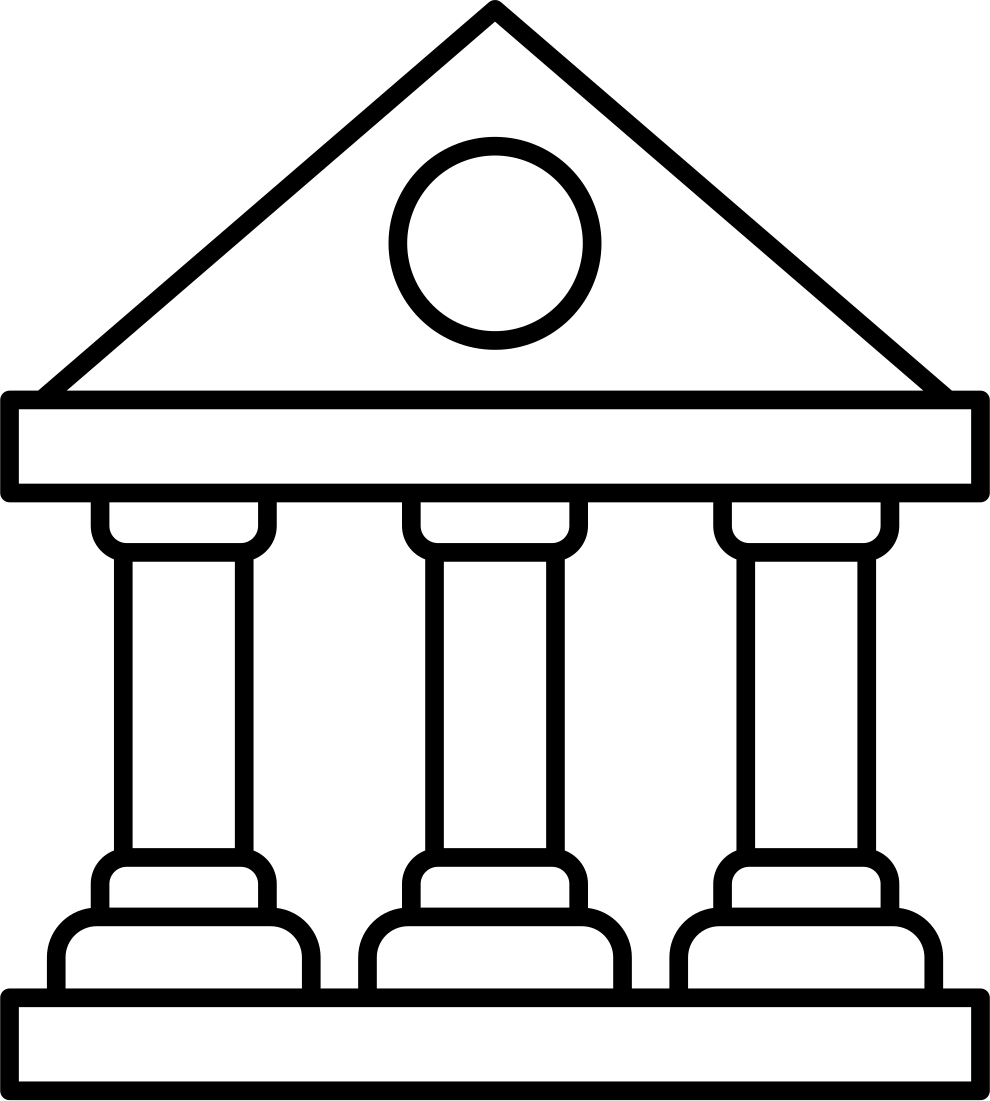
\includegraphics[width=1cm]{clipart/bank}
\index{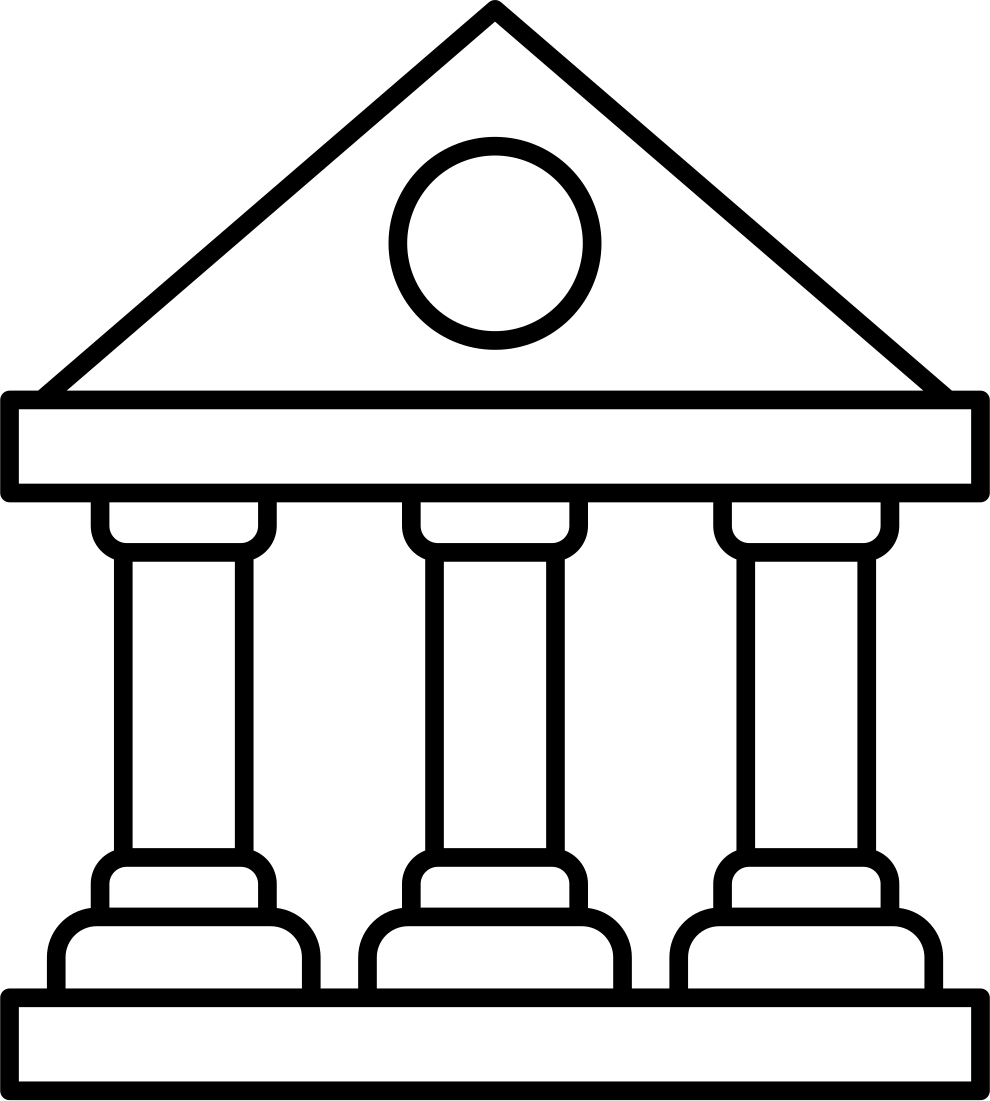
\includegraphics[height=3mm]{clipart/bank}\href{https://thenounproject.com/icon/bank-1561550/}{Bank} by \href{https://thenounproject.com/back1design1/}{Cuby Design} is licensed under \CCBYthree~(accessed 28 August 2022) }
}

\pause
If one interest payment comes at time $t$, then the next interest payment will be made at time $t+\frac{1}{n}$
and will be: \[\frac{1}{n}\times\frac{r}{100}\times B(t)=\frac{r}{100n}B(t)\]

\onslide<3->{
So, calling $\frac{1}{n}=h$,
\begin{equation*}
B(t+h)=B(t) + \frac{r}{100}B(t)h\qquad\text{or}\qquad
\frac{B(t+h)-B(t)}{h} = \frac{r}{100}B(t)
\end{equation*}

If the interest is compounded continuously,
\begin{align*}
\diff{B}{t}(t)&=\lim_{h\rightarrow 0}\frac{B(t+h)-B(t)}{h} = \frac{r}{100}B(t)\\
\implies  B(t)&=B(0)\cdot e^{rt/100}=P\cdot e^{rt/100}
\end{align*}
}
\unote{Example~\eref{text}{eg:SDEmoneyA}}
\end{frame}
%----------------------------------------------------------------------------------------
\begin{frame}[t]
\begin{block}{Continuously compounding interest}
If an account with balance $B(t)$ pays a continuously compounding rate of $r$\% per year, then:
\begin{align*}
\diff{B}{t}&=\frac{r}{100}B\\
B(t)&=B(0)\cdot e^{rt/100}
\end{align*}
\end{block}
\end{frame}
%----------------------------------------------------------------------------------------
\begin{frame}[t]
\AnswerYes<1>
\label{note2.4.2d}
You invest \$200\,000 into an account with continuously compounded interest of 5\% annually. 
You want to withdraw from the account continuously at a rate of \$$W$ per year, for the next 20 years. How big can $W$ be? 
\vfill

\sonslide<2>{
Let $A(t)$ be the balance in the account $t$ years after the initial deposit.
	\begin{align*}
	\diff{A}{t}&=\frac{5}{100}A-W=\frac{1}{20}\left(A-20W\right)\\
	A(t)&=(200\,000-20W)e^{t/20}+20W\\
	0=A(20)&=(200\,000-20W)e+20W\\
	&=200\,000 e +20W(1-e)\\
	W&=\frac{200\,000e }{20(e-1)}=10\,000 \frac{e}{e-1}\approx15\,819.77
	\end{align*}

That is, you can withdraw $10\,000 \frac{e}{e-1}\approx15\,819.77$ each year.
}

\unote{Example~\eref{text}{eg:SDEmoneyC}}
\end{frame}
%----------------------------------------------------------------------------------------
%----------------------------------------------------------------------------------------
%----------------------------------------------------------------------------------------
%----------------------------------------------------------------------------------------

